\section{Exercices d'application}

\rubrique{Limites à l'infini et limites finies}

\exo{}\diff{1}
Déterminer les limites suivantes :
\[
\lim_{x\to +\infty} (3x^2-5x+2),\qquad 
\lim_{x\to -\infty} (-2x^3+4x-1),\qquad 
\lim_{x\to +\infty} \frac{5x+3}{2x-1}.
\]

\exo{}\diff{1}
Calculer les limites suivantes :
\[
\lim_{x\to -\infty} \frac{2x^2-3x+1}{x^2+4},\qquad 
\lim_{x\to +\infty} \frac{-3x+2}{\sqrt{x}}.
\]

\exo{}\diff{2}
Soit $f$ la fonction définie sur $\R\setminus\{1\}$ par $f(x)=\dfrac{x^2-3x+2}{x-1}$.
\begin{enumerate}[label=\alph*)]
\item Simplifier $f(x)$ pour $x\neq 1$.
\item En déduire $\displaystyle\lim_{x\to 1} f(x)$.
\end{enumerate}

\rubrique{Formes indéterminées}

\exo{}\diff{2}
Déterminer les limites suivantes en levant l'indétermination :
\[
\lim_{x\to +\infty} (\sqrt{x+1}-\sqrt{x}),\qquad 
\lim_{x\to 2} \frac{x^2-4}{x-2}.
\]

\exo{}\diff{2}
Calculer $\displaystyle\lim_{x\to +\infty} \frac{3x^2-2x+1}{-x^2+5x-3}$ et $\displaystyle\lim_{x\to -\infty} \frac{2x^3-5x}{x^2+1}$.

\rubrique{Continuité}

\exo{}\diff{1}
La fonction $f$ définie sur $\R$ par $f(x)=x^3-2x+1$ est-elle continue en $x=0$ ? Justifier.

\exo{}\diff{2}
On considère la fonction $g$ définie sur $\R$ par :
\[
g(x)=\begin{cases}
x^2+1 &\text{si } x\leq 2,\\
5x-5 &\text{si } x>2.
\end{cases}
\]
Étudier la continuité de $g$ en $x=2$.

\exo{}\diff{3}
Soit $h$ la fonction définie sur $\R$ par $h(x)=\dfrac{x^2-1}{|x-1|}$ pour $x\neq 1$ et $h(1)=2$.
Étudier la continuité de $h$ en $x=1$.

\rubrique{Asymptotes}

\exo{}\diff{2}
Soit $f(x)=\dfrac{2x+1}{x-3}$.
\begin{enumerate}[label=\alph*)]
\item Déterminer les limites de $f$ aux bornes de son ensemble de définition.
\item En déduire les équations des asymptotes à la courbe de $f$.
\end{enumerate}

\exo{}\diff{2}
Soit $g(x)=\dfrac{x^2+1}{x}$.
\begin{enumerate}[label=\alph*)]
\item Déterminer $\displaystyle\lim_{x\to 0^+} g(x)$ et $\displaystyle\lim_{x\to 0^-} g(x)$.
\item Montrer que la droite d'équation $y=x$ est asymptote oblique à la courbe de $g$ en $+\infty$ et $-\infty$.
\end{enumerate}

\section{Exercices d'entraînement}

\rubrique{Limites à l'infini et limites finies}

\exo{}\diff{1}
Calculer : $\displaystyle\lim_{x\to +\infty} (5-2x)$, $\displaystyle\lim_{x\to -\infty} (x^2+3x-7)$, $\displaystyle\lim_{x\to +\infty} \frac{4}{x+2}$.

\exo{}\diff{1}
Déterminer $\displaystyle\lim_{x\to 3} (2x-1)$ et $\displaystyle\lim_{x\to -1} (x^2+4x)$.

\exo{}\diff{2}
Soit $f(x)=\dfrac{3x-2}{x+4}$. Calculer les limites de $f$ en $+\infty$, $-\infty$, $-4^+$ et $-4^-$.

\exo{}\diff{2}
Calculer $\displaystyle\lim_{x\to +\infty} \frac{2x^2-3x+5}{x^2+2x-1}$ et $\displaystyle\lim_{x\to -\infty} \frac{-x^3+2x}{x^2-1}$.

\exo{}\diff{2}
Déterminer $\displaystyle\lim_{x\to +\infty} (\sqrt{x^2+2x}-x)$.

\rubrique{Formes indéterminées}

\exo{}\diff{2}
Calculer $\displaystyle\lim_{x\to 1} \frac{x^2-1}{x-1}$ et $\displaystyle\lim_{x\to -2} \frac{x^2+3x+2}{x+2}$.

\exo{}\diff{2}
Déterminer $\displaystyle\lim_{x\to +\infty} \frac{4x^3-2x+1}{-2x^3+5x^2}$ et $\displaystyle\lim_{x\to -\infty} \frac{3x^2-5x}{x+2}$.

\exo{}\diff{3}
Soit $f(x)=\dfrac{\sqrt{x+1}-1}{x}$. Calculer $\displaystyle\lim_{x\to 0} f(x)$.

\exo{}\diff{3}
Calculer $\displaystyle\lim_{x\to +\infty} (\sqrt{x^2+3x+1}-x)$.

\rubrique{Continuité}

\exo{}\diff{1}
La fonction $f(x)=2x-3$ est-elle continue sur $\R$ ? Justifier.

\exo{}\diff{2}
Étudier la continuité en $x=1$ de la fonction $g$ définie par :
\[
g(x)=\begin{cases}
x+2 &\text{si } x<1,\\
3x &\text{si } x\geq 1.
\end{cases}
\]

\exo{}\diff{2}
Soit $h(x)=\dfrac{x^2-4}{x-2}$ pour $x\neq 2$ et $h(2)=4$. $h$ est-elle continue en $2$ ?

\exo{}\diff{3}
Déterminer $a\in\R$ pour que la fonction $f$ définie par :
\[
f(x)=\begin{cases}
ax+1 &\text{si } x\leq 2,\\
x^2-3 &\text{si } x>2,
\end{cases}
\]
soit continue en $x=2$.

\rubrique{Asymptotes}

\exo{}\diff{2}
Soit $f(x)=\dfrac{3x-1}{x+2}$. Déterminer les asymptotes de sa courbe.

\exo{}\diff{2}
Soit $g(x)=\dfrac{2x^2-3x+1}{x-1}$. Montrer que la droite $y=2x-1$ est asymptote oblique à la courbe de $g$ en $+\infty$ et $-\infty$.

\exo{}\diff{3}
Soit $h(x)=\dfrac{x^3-2x^2+1}{x^2}$. Déterminer les asymptotes éventuelles.

\section{Problèmes type Probatoire/Bac}

\sujetbac[Limites et continuité d'une fonction rationnelle]
Soit $f$ la fonction définie sur $\R\setminus\{2\}$ par $f(x)=\dfrac{x^2-3x+1}{x-2}$.
\begin{enumerate}[label=\arabic*)]
\item Déterminer les limites de $f$ aux bornes de son ensemble de définition.
\item Montrer que la droite $D: y=x-1$ est asymptote oblique à la courbe $C_f$ de $f$ en $+\infty$ et $-\infty$.
\item Étudier la position relative de $C_f$ et $D$.
\item La fonction $f$ est-elle prolongeable par continuité en $x=2$ ? Justifier.
\end{enumerate}

\sujetbac[Étude d'une fonction avec paramètre]
On considère la fonction $g$ définie sur $\R$ par :
\[
g(x)=\begin{cases}
x^2+ax+b &\text{si } x\leq 1,\\
\dfrac{2x-1}{x} &\text{si } x>1.
\end{cases}
\]
\begin{enumerate}[label=\arabic*)]
\item Déterminer $a$ et $b$ pour que $g$ soit continue en $x=1$.
\item Pour $a=2$ et $b=-1$, étudier la continuité de $g$ sur $\R$.
\item Calculer $\displaystyle\lim_{x\to +\infty} g(x)$ et $\displaystyle\lim_{x\to -\infty} g(x)$.
\end{enumerate}

\sujetbac[Lecture graphique et limites]
On donne ci-dessous la courbe d'une fonction $f$ définie sur $\R\setminus\{-1\}$.
\begin{illus}
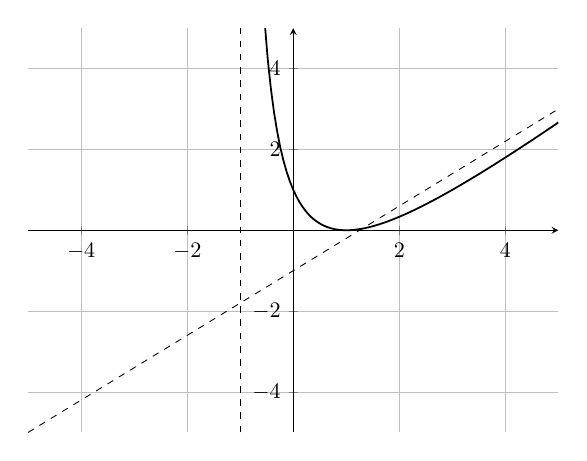
\begin{tikzpicture}[scale=0.8]
\begin{axis}[axis lines=center, xmin=-5, xmax=5, ymin=-5, ymax=5, samples=100, grid=both, width=10cm, height=8cm]
\addplot[thick, domain=-5:-1.1] {(x^2-2*x+1)/(x+1)};
\addplot[thick, domain=-0.9:5] {(x^2-2*x+1)/(x+1)};
\addplot[dashed] coordinates {(-1,-5) (-1,5)};
\addplot[dashed] coordinates {(-5,-5) (5,3)};
\end{axis}
\end{tikzpicture}
\fig{Courbe de $f$}
\end{illus}
\begin{enumerate}[label=\arabic*)]
\item Lire graphiquement :
\begin{enumerate}[label=\alph*)]
\item $\displaystyle\lim_{x\to -\infty} f(x)$ et $\displaystyle\lim_{x\to +\infty} f(x)$.
\item $\displaystyle\lim_{x\to -1^-} f(x)$ et $\displaystyle\lim_{x\to -1^+} f(x)$.
\end{enumerate}
\item Donner l'équation de l'asymptote verticale et de l'asymptote oblique.
\item Retrouver ces résultats par le calcul sachant que $f(x)=\dfrac{x^2-2x+1}{x+1}$.
\end{enumerate}

\section{Corrigés}

\corrige{de l'exercice 1}
\begin{enumerate}[label=\alph*)]
\item $\displaystyle\lim_{x\to +\infty} (3x^2-5x+2)=\lim_{x\to +\infty} 3x^2=+\infty$.
\item $\displaystyle\lim_{x\to -\infty} (-2x^3+4x-1)=\lim_{x\to -\infty} -2x^3=+\infty$ (car $x^3\to -\infty$ et $-2\times(-\infty)=+\infty$).
\item $\displaystyle\lim_{x\to +\infty} \frac{5x+3}{2x-1}=\lim_{x\to +\infty} \frac{5x}{2x}=\frac{5}{2}$.
\end{enumerate}

\corrige{de l'exercice 2}
\begin{enumerate}[label=\alph*)]
\item $\displaystyle\lim_{x\to -\infty} \frac{2x^2-3x+1}{x^2+4}=\lim_{x\to -\infty} \frac{2x^2}{x^2}=2$.
\item $\displaystyle\lim_{x\to +\infty} \frac{-3x+2}{\sqrt{x}}=\lim_{x\to +\infty} \frac{-3x}{\sqrt{x}}=\lim_{x\to +\infty} -3\sqrt{x}=-\infty$.
\end{enumerate}

\corrige{de l'exercice 3}
\begin{enumerate}[label=\alph*)]
\item $f(x)=\dfrac{x^2-3x+2}{x-1}=\dfrac{(x-1)(x-2)}{x-1}=x-2$ pour $x\neq 1$.
\item $\displaystyle\lim_{x\to 1} f(x)=\lim_{x\to 1} (x-2)=-1$.
\end{enumerate}

\corrige{de l'exercice 4}
\begin{enumerate}[label=\alph*)]
\item $\sqrt{x+1}-\sqrt{x}=\dfrac{(x+1)-x}{\sqrt{x+1}+\sqrt{x}}=\dfrac{1}{\sqrt{x+1}+\sqrt{x}}\to 0$ quand $x\to +\infty$.
\item $\dfrac{x^2-4}{x-2}=\dfrac{(x-2)(x+2)}{x-2}=x+2$ pour $x\neq 2$, donc $\displaystyle\lim_{x\to 2} \frac{x^2-4}{x-2}=4$.
\end{enumerate}

\corrige{de l'exercice 5}
\begin{enumerate}[label=\alph*)]
\item $\displaystyle\lim_{x\to +\infty} \frac{3x^2-2x+1}{-x^2+5x-3}=\lim_{x\to +\infty} \frac{3x^2}{-x^2}=-3$.
\item $\displaystyle\lim_{x\to -\infty} \frac{2x^3-5x}{x^2+1}=\lim_{x\to -\infty} \frac{2x^3}{x^2}=\lim_{x\to -\infty} 2x=-\infty$.
\end{enumerate}

\corrige{de l'exercice 6}
$f$ est une fonction polynôme, donc continue sur $\R$. En particulier, elle est continue en $x=0$. On vérifie : $f(0)=1$ et $\displaystyle\lim_{x\to 0} f(x)=1$.

\corrige{de l'exercice 7}
Calculons $\displaystyle\lim_{x\to 2^-} g(x)=\lim_{x\to 2^-} (x^2+1)=5$ et $\displaystyle\lim_{x\to 2^+} g(x)=\lim_{x\to 2^+} (5x-5)=5$. De plus $g(2)=2^2+1=5$. Donc $\displaystyle\lim_{x\to 2} g(x)=g(2)=5$, donc $g$ est continue en $2$.

\corrige{de l'exercice 8}
Pour $x\neq 1$, $|x-1|=\begin{cases} x-1 &\text{si } x>1,\\ 1-x &\text{si } x<1. \end{cases}$
Donc pour $x>1$, $h(x)=\dfrac{x^2-1}{x-1}=x+1$ ; pour $x<1$, $h(x)=\dfrac{x^2-1}{1-x}=-(x+1)$.
Ainsi $\displaystyle\lim_{x\to 1^+} h(x)=2$ et $\displaystyle\lim_{x\to 1^-} h(x)=-2$. Les limites à gauche et à droite sont différentes, donc $h$ n'est pas continue en $1$ (même si $h(1)=2$).

\corrige{de l'exercice 9}
\begin{enumerate}[label=\alph*)]
\item $D_f=\R\setminus\{3\}$. $\displaystyle\lim_{x\to +\infty} f(x)=\lim_{x\to +\infty} \frac{2x}{x}=2$, $\displaystyle\lim_{x\to -\infty} f(x)=2$. $\displaystyle\lim_{x\to 3^-} f(x)=\lim_{x\to 3^-} \frac{2x+1}{x-3}=-\infty$ (car numérateur $\to 7>0$, dénominateur $\to 0^-$), $\displaystyle\lim_{x\to 3^+} f(x)=+\infty$.
\item Asymptote horizontale $y=2$ en $+\infty$ et $-\infty$ ; asymptote verticale $x=3$.
\end{enumerate}

\corrige{de l'exercice 10}
\begin{enumerate}[label=\alph*)]
\item $\displaystyle\lim_{x\to 0^+} g(x)=\lim_{x\to 0^+} \left(x+\frac{1}{x}\right)=+\infty$, $\displaystyle\lim_{x\to 0^-} g(x)=-\infty$.
\item $g(x)-x=\dfrac{1}{x}\to 0$ quand $x\to \pm\infty$, donc $y=x$ est asymptote oblique.
\end{enumerate}

\corrige{du problème 1}
\begin{enumerate}[label=\arabic*)]
\item $D_f=\R\setminus\{2\}$. $\displaystyle\lim_{x\to +\infty} f(x)=\lim_{x\to +\infty} \frac{x^2}{x}=+\infty$, $\displaystyle\lim_{x\to -\infty} f(x)=-\infty$. $\displaystyle\lim_{x\to 2^-} f(x)=\lim_{x\to 2^-} \frac{4-6+1}{0^-}=\frac{-1}{0^-}=+\infty$, $\displaystyle\lim_{x\to 2^+} f(x)=-\infty$.
\item $f(x)-(x-1)=\dfrac{x^2-3x+1}{x-2}-(x-1)=\dfrac{x^2-3x+1-(x-1)(x-2)}{x-2}=\dfrac{x^2-3x+1-(x^2-3x+2)}{x-2}=\dfrac{-1}{x-2}\to 0$ en $\pm\infty$, donc $D$ est asymptote oblique.
\item Le signe de $f(x)-(x-1)=-\dfrac{1}{x-2}$ : si $x>2$, $f(x)-(x-1)<0$ donc $C_f$ est en dessous de $D$ ; si $x<2$, $f(x)-(x-1)>0$ donc $C_f$ est au-dessus de $D$.
\item $\displaystyle\lim_{x\to 2} f(x)$ n'existe pas (limites infinies différentes), donc $f$ n'est pas prolongeable par continuité en $2$.
\end{enumerate}

\corrige{du problème 2}
\begin{enumerate}[label=\arabic*)]
\item Continuité en $1$ : $\displaystyle\lim_{x\to 1^-} g(x)=1+a+b$, $\displaystyle\lim_{x\to 1^+} g(x)=\frac{2-1}{1}=1$, et $g(1)=1+a+b$. On doit avoir $1+a+b=1$, donc $a+b=0$.
\item Pour $a=2$, $b=-1$, on a $a+b=1\neq 0$, donc $g$ n'est pas continue en $1$ (car $\displaystyle\lim_{x\to 1^-} g(x)=2\neq 1$). Sur $]-\infty,1[$ et $]1,+\infty[$, $g$ est continue (polynôme et quotient de polynômes). Donc $g$ est continue sur $\R\setminus\{1\}$.
\item $\displaystyle\lim_{x\to +\infty} g(x)=\lim_{x\to +\infty} \frac{2x-1}{x}=2$, $\displaystyle\lim_{x\to -\infty} g(x)=\lim_{x\to -\infty} (x^2+2x-1)=+\infty$.
\end{enumerate}

\corrige{du problème 3}
\begin{enumerate}[label=\arabic*)]
\item Par lecture graphique : $\displaystyle\lim_{x\to -\infty} f(x)=-\infty$, $\displaystyle\lim_{x\to +\infty} f(x)=+\infty$, $\displaystyle\lim_{x\to -1^-} f(x)=-\infty$, $\displaystyle\lim_{x\to -1^+} f(x)=+\infty$.
\item Asymptote verticale $x=-1$, asymptote oblique $y=x-3$ (d'après le graphique).
\item Par le calcul : $f(x)=\dfrac{x^2-2x+1}{x+1}$. En $+\infty$, $\displaystyle\lim_{x\to +\infty} f(x)=+\infty$ ; en $-\infty$, $-\infty$. $f(x)-(x-3)=\dfrac{x^2-2x+1-(x-3)(x+1)}{x+1}=\dfrac{x^2-2x+1-(x^2-2x-3)}{x+1}=\dfrac{4}{x+1}\to 0$, donc $y=x-3$ est asymptote oblique. $\displaystyle\lim_{x\to -1^-} f(x)=-\infty$ (numérateur $\to 4>0$, dénominateur $\to 0^-$), $\displaystyle\lim_{x\to -1^+} f(x)=+\infty$, donc $x=-1$ est asymptote verticale.
\end{enumerate}